\section{Introduction} % (fold)
\label{sec:introduction}

\HG is a interactive website designed for people who want to get an overview of history. The appear of this events in function of time on the map helps you to get an impression of the behave of history.

With \HG there is much less need of unwieldy things like big maps of historical places or books and many piece of paper. Everyone should be able to learn our past in a nice, intuitive and simple way to be prepared for future.

\begin{figure}[H]
	\centering
	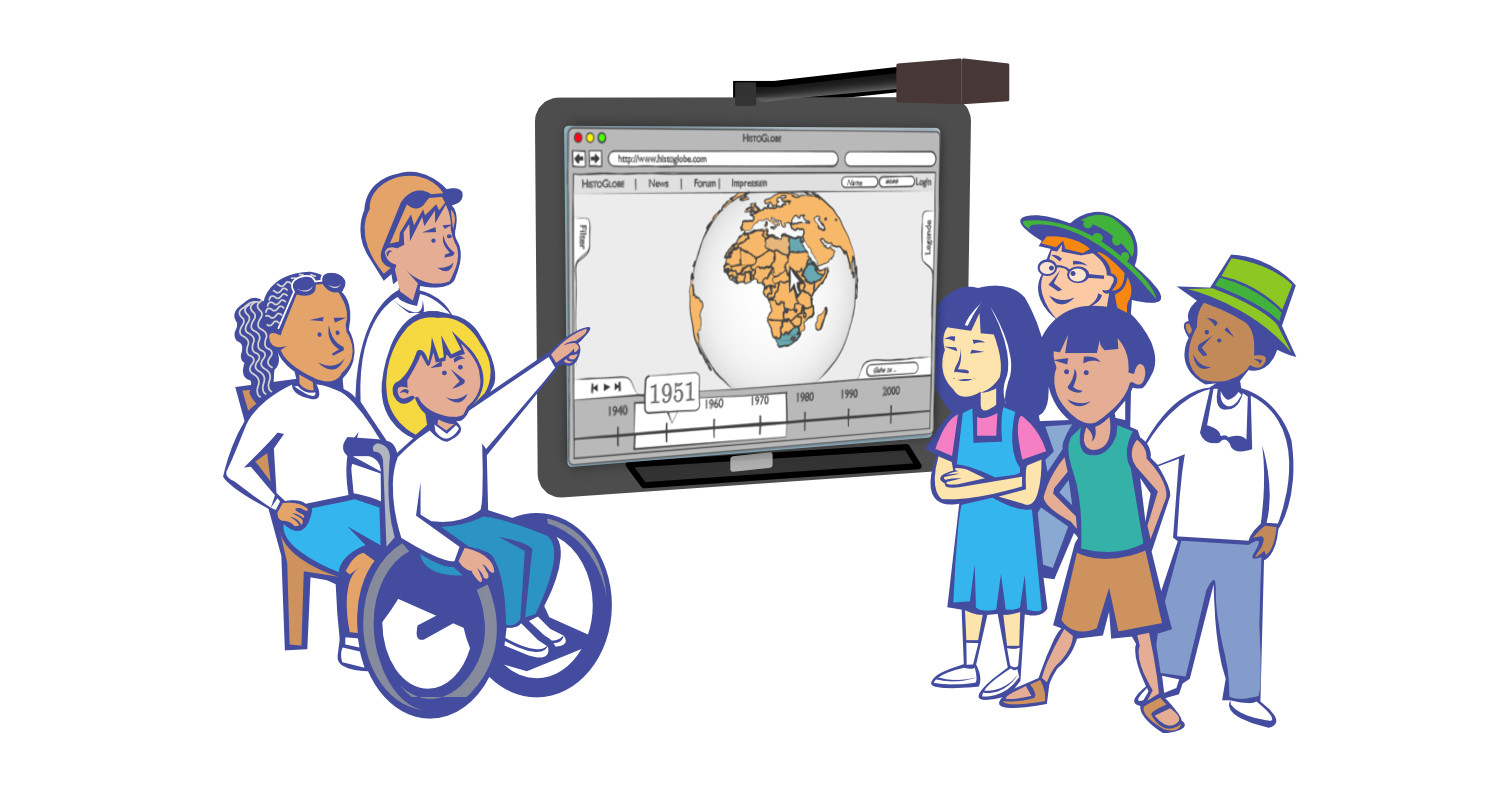
\includegraphics[width=0.8\textwidth]{graphics/everybody.jpg}
	\caption{Interactive Learning with \textsc{HistoGlobe}}
	\label{fig:everybody}
\end{figure}

We combined the geographical and chronological dimensions of history in one interface. This allows us to combine most things you need to teach. The combination of time and place helps you to understand the relation of historical events.

So we are able to present students in school our way to figure out history, guided by teachers or on their own.
\\
\\
This is \textsc{HistoGlobe}!

% section introduction (end)
